\chapter{Tutorials}
\label{chap:tuto}
This tutorial will teach you how to use \faust with \ros through the turtlesim package.

\section{DSP File}
Copy the following code into a text file and save it as \lstinline'roscillator.dsp'.

\begin{lstlisting}
declare name 		"roscillator";
declare version 	"1.0";
declare author 		"Grame";
declare license 	"BSD";
declare copyright 	"(c)GRAME 2009";

//-----------------------------------------------
// 			Sinusoidal Oscillator
//-----------------------------------------------

import("music.lib");

smooth(c) = *(1-c) : +~*(c);
vol = hslider("volume [unit:dB][ros:/turtle1/pose turtlesim Pose x 0.0 11.0]", 0, -96, -96, 0.1) : db2linear : smooth(0.999) ;
freq = hslider("freq [unit:Hz][ros:/turtle1/pose turtlesim Pose y 0.0 11.0]", 1000, 20, 24000, 1);


process = vgroup("Oscillator", osc(freq) * vol);

\end{lstlisting}

\newpage

\section{Compilation}
\subsection{If you installed FAUST on your machine}
In a terminal, type :
\begin{lstlisting}
faust2rosgtk -install ~/catkin_ws ~/path/to/roscillator.dsp
\end{lstlisting}
The compilation can take between 10 and 15 seconds.
Then, go in your workspace's root and source the setup file (see section \ref{sec:rostips})

\subsection{With FaustLive}
FaustLive is available on \href{https://sourceforge.net/projects/faudiostream/files/}
{Source Forge}. Once FaustLive installed, launch it.\\
Choose \texttt{Open your File.dsp} and select \texttt{roscillator.dsp}. The file 
will be compiled and executed. 
To export it, clic on \texttt{Window/Export As...} or press \texttt{Ctrl+P}. The Export 
Manager window should be opened.

\begin{figure}[ht!]
\centering
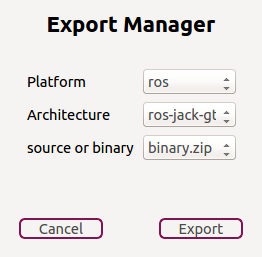
\includegraphics[scale=0.5]{images/faustlive-export.png}
\caption{FaustLive Export Manager}
\label{fig:welcomefaustlive}
\end{figure}

Select \texttt{ros} as platform, \texttt{ros-jack-gtk} as architecture, and \texttt{binary.zip} 
as binary. Then click on \texttt{Export}, and \texttt{Save}. \\
Unzip your package in your current \ros workspace, and make your workspace with 
\texttt{catkin\_make}, and source it (see the \ros tips in section \ref{sec:rostips}).

%\begin{figure}[ht!]
%\centering
%\includegraphics[scale=0.2]{images/faustlive-welcome.png}
%\caption{FaustLive interface}
%\label{fig:welcomefaustlive}
%\end{figure}

\subsection{With the online compiler}
The online compiler is available on \href{http://faust.grame.fr/index.php/online-examples}{the 
\faust Website}. In \texttt{Faust Code} tab, drop your roscillator.dsp file.  In the 
\texttt{Exec File} tab, choose \texttt{Ros ros-jack-gtk} as architecture, and click on 
\texttt{Download the executable file}.\\
Unzip your package in your current \ros workspace, make your workspace with 
\texttt{catkin\_make}, and source it (see the \ros tips in section \ref{sec:rostips}).

\newpage

\section{Run}
In a terminal, run the master : 
\begin{lstlisting}
roscore
\end{lstlisting}
In two new terminals, run the turtlesim node and the teleop\_key node :
\begin{lstlisting}
rosrun turtlesim turtlesim_node
\end{lstlisting}
\begin{lstlisting}
rosrun turtlesim turtle_teleop_key
\end{lstlisting}
In a fourth (and last) terminal, run your \faust node :
\begin{lstlisting}
rosrun roscillator_gtk roscillator_gtk
\end{lstlisting}
You should have four open terminals, a turtle window, and a \faust window.

\begin{figure}[ht!]
\centering
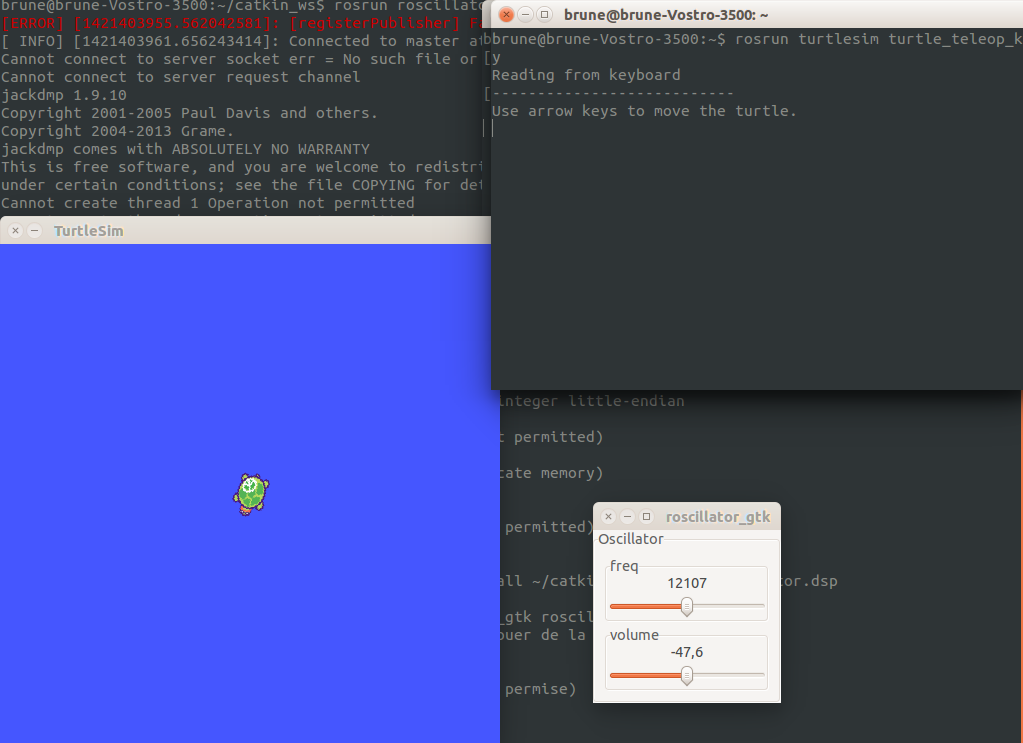
\includegraphics[scale=0.2]{images/tutocommandline.png}
\caption{Screenshot with the four open terminals}
\label{fig:screenshot}
\end{figure}

\subsection{Use}
To move your turtle, go back on the teleop\_key terminal and use your arrow keys.

\newpage

\section{ROS tips}
\label{sec:rostips}
\subsection{How to create a ROS workspace ?} 
\begin{lstlisting}
mkdir -p ~/catkin_ws/src
cd ~/catkin_ws/src
catkin_init_workspace
\end{lstlisting}
\subsection{How to make your workspace ?}
\begin{lstlisting}
cd ~/catkin_ws
catkin_make
\end{lstlisting}
\subsection{How to source a workspace ?}
\begin{lstlisting}
cd ~/catkin_ws
source devel/setup.bash
\end{lstlisting}